%%%%%%%%%%%%%%%%%%%%%%%%%%%%%%%%%%%%%%%%%%%%%%%%%%%%%%%%%%%%%%%%%%%%%%
% If you're new to LaTeX, the wikibook is a great place to start:
% http://en.wikibooks.org/wiki/LaTeX
%
%%%%%%%%%%%%%%%%%%%%%%%%%%%%%%%%%%%%%%%%%%%%%%%%%%%%%%%%%%%%%%%%%%%%%%
% Edit the title below to update the display in My Documents
\title{Project Intranet Allpower}
%
%%% Preamble
\documentclass[a4paper,11pt,twoside,titlepage,openright]{report}
\usepackage[T1]{fontenc}
\usepackage{fourier}
\usepackage[utf8]{inputenc}
\usepackage[titles]{tocloft}
\cftsetindents{figure}{0em}{3.5em}
\cftsetindents{table}{0em}{3.5em}

% Glossarey
\usepackage[toc]{glossaries}
\makeglossaries
\usepackage{xparse}
\DeclareDocumentCommand{\entry}{ O{} O{} m m m m} {
  \newglossaryentry{gls-#3}{name={#5},text={#5\glsadd{#3}},
    description={#6},#1
  }
  \makeglossaries
  \newacronym[see={[Siehe:]{gls-#3}},#2]{#3}{#4}{#5\glsadd{gls-#3}}
}


\newglossaryentry{defacement}
{
  name=Defacement,
  description={(engl. für „Entstellung“ oder „Verunstaltung“) bezeichnet das unberechtigte Verändern einer Website}
}

\newglossaryentry{frontend}
{
	name=Front End,
    description={die der Öffentlichkeit zugänglichen Internetseiten}
}

\newglossaryentry{backend}
{
	name=Back End,
    description={die Administrationsoberfläche zum Erstellen und Pflegen von Inhalten einer Webseite}
}

\newglossaryentry{unix}
{
	name=UNIX,
    description={universell einsetzbares, besonders leistungsfähiges Betriebssystem}
}

\newglossaryentry{linux}
{
	name=Linux,
    description={freies Betriebssystem, das \gls{unix} basierend ist}
}

\newglossaryentry{widget}
{
	name=Widget,
    description={kleines Computerprogramm, das in ein anderes Programm integriert wird, besonders als Teil einer grafischen Benutzeroberfläche}
}

\newglossaryentry{zip}
{
	name=ZIP,
    description={ein Format für verlustfrei komprimierte Dateien}
}

\newglossaryentry{opensource}
{
	name={Open Source},
    description={Software bezeichnet, deren Quelltext öffentlich und von Dritten eingesehen werden kann}
}

\entry{pixel}{px}{Pixel}{von Picture Element, Bildelement}{}
\entry{tinymce}{TinyMCE}{Tiny Moxiecode Content Editor}{Editor für Webanwendungen}
\entry{ip}{IP}{Internet Protocol}{in Computernetzen weit verbreitetes Netzwerkprotokoll, stellt die Grundlage des Internets dar}
\entry{php}{PHP}{PHP: Hypertext Preprocessor}{eine Skriptsprache, die hauptsächlich zur Erstellung dynamischer Webseiten oder Webanwendungen verwendet wird}
\entry{html}{HTML}{Hypertext Markup Language}{eine textbasierte Auszeichnungssprache zur Strukturierung digitaler Dokumente wie Texte mit Hyperlinks, Bildern und anderen Inhalten}
\entry{css}{CSS}{Cascade Style Sheet}{eine Computersprache für die Gestaltung digitaler, vorwiegend Web-basierter Dokumente}
\entry{cms}{CMS}{Content Management System}{eine Software zur gemeinschaftlichen Bearbeitung von ''Inhalten'' (Content), zumeist in Webseiten}
\entry{sql}{SQL}{Structured Query Language}{eine Datenbanksprache zur Definition von Datenstrukturen in relationalen Datenbanken sowie zum Bearbeiten (Einfügen, Verändern, Löschen) und Abfragen von darauf basierenden Datenbeständen}
\entry{http}{HTTP}{Hypertext Transfer Protocol}{ein Anwendungsprotokoll zur Übertragung von Daten über ein Netzwerk}
\entry{iis}{IIS}{Internet Information Services}{ein erweiterbarer Webserver für Windows}
\entry{rss}{RSS}{Rich Site Summary}{eine Technologie zum Abonnement von Webseiten-Inhalten}
\entry{www}{WWW}{World Wide Web}{ein über das Internet abrufbares System von elektronischen Hypertext-Dokumenten}
\entry{ldap}{LDAP}{Lightweight Directory Access Protocol}{ein Netzwerkprotokoll zur Abfrage und Änderung von Informationen verteilter Verzeichnisdienste}
\entry{gif}{GIF}{Grafics Interchange Format}{ein Grafikformat für Bilder mit Farbpalette}
\entry{png}{PNG}{Portable Network Graphics}{en Grafikformat, das als Ersatz für das Format GIF entworfen wurde}
\entry{wysiwyg}{WYSIWIG}{What You See Is What You Get}{bei WYSIWYG wird ein Dokument während der Bearbeitung am Bildschirm genauso angezeigt, wie es bei der Ausgabe über ein anderes Gerät, z. B. einen Drucker, aussieht}
\entry{ftp}{FTP}{File Transfer Protocol}{ein Netzwerkprotokoll zur Dateiübertragung}
\entry{pdf}{PDF}{Portable Document Format}{ein plattformunabhängiges Dateiformat für Dokumente}
\entry{rwd}{RWD}{responsives Webdesign}{ein gestalterisches und technisches Muster zur Erstellung von Websites, so dass diese auf Eigenschaften des jeweils benutzten Endgeräts, vor allem Smartphones und Tabletcomputer, reagieren können}
\entry{url}{URL}{Uniform Resource Locator}{identifiziert und lokalisiert eine Ressource, beispielsweise eine Website über die zu verwendende Zugriffsmethode (zum Beispiel das verwendete Netzwerkprotokoll wie \acrshort{http} oder \acrshort{ftp}) und den Ort der Ressource in Computernetzwerken}

\widowpenalty=10000
\clubpenalty=10000


% German language/hyphenation
\usepackage[ngerman]{babel}
\usepackage[protrusion=true,expansion=true]{microtype}	
\usepackage{amsmath,amsfonts,amsthm} % Math packages
\usepackage[pdftex]{graphicx}	
\usepackage{url}
\linespread{1.3}
\hyphenation{MySQL PostgreSQL MariaDB miniOrange Joomla Typo TinyMCE ldap}
\usepackage{listings}
\usepackage{pifont}

% Diagramme
\usepackage{pgfplots}
\pgfplotsset{compat=1.12}

% Captions
\RequirePackage[labelsep=space,tableposition=top]{caption}

%%% Custom sectioning
\usepackage{sectsty}
\allsectionsfont{\normalfont\scshape}

%Table
\usepackage{booktabs}
\usepackage{multirow}

\usepackage{float}
\usepackage{wrapfig}
\usepackage{subcaption}

%%% Custom headers/footers (fancyhdr package)
\usepackage{fancyhdr}
\pagestyle{fancyplain}
\fancyhead[LE]{\leftmark}
\fancyhead[LO]{}
\fancyhead[C]{}
\fancyhead[RE]{}
\fancyhead[RO]{\rightmark}

\fancyfoot[LE]{\thepage}
\fancyfoot[C]{}
\fancyfoot[RO]{\thepage}
\renewcommand{\headrulewidth}{0pt}		% Remove header underlines
\renewcommand{\footrulewidth}{0pt}		% Remove footer underlines
\setlength{\headheight}{13.6pt}


%%% Equation and float numbering
\numberwithin{equation}{section}		% Equationnumbering: section.eq#
\numberwithin{figure}{section}			% Figurenumbering: section.fig#
\numberwithin{table}{section}				% Tablenumbering: section.tab#



%%% Maketitle metadata
\newcommand{\horrule}[1]{\rule{\linewidth}{#1}} 	% Horizontal rule

\title{
		%\vspace{-1in} 	
		\usefont{OT1}{bch}{b}{n}
%		\normalfont \normalsize \textsc{School of random department names} \\ [25pt]
		\horrule{0.5pt} \\[0.4cm]
		\huge Projekt: Intranet Allpower \\
		\horrule{2pt} \\[0.5cm]
}
\author{
		\normalfont
        \normalsize
        Christian Seiler\\[-3pt]
        christian@christianseiler.ch\\
        \\
        \normalsize
        \\
        \\
        \\
}
\date{M\"{a}rz - Juni 2016}


%%% Begin document
\begin{document}
\maketitle

\pagenumbering{roman}
\tableofcontents
\clearpage
\listoffigures
\clearpage
\listoftables
\clearpage

\pagenumbering{arabic}
\chapter{Einführung}
\section{Allgemeine Informationen}
Als Intranet wird eine Website bezeichnet, welche typischerweise nur innerhalb eines Unternehmens zugänglich ist. Ziele eines Intranets sind unter anderem:

\begin{itemize}
\item konzentrierte Informationsweitergabe an die Mitarbeiter
\item zentrale Datenbank für die wichtigsten Dokumente und Daten
\item Übersicht aller Mitarbeiter
\item stärkeres betriebsinternes Zugehörigkeitsgefühl (Corporate Design, Corporate Identity)
\end{itemize}

Die Struktur und der Inhalt eines Intranet variiert stark nach den Bedürfnissen eines Unternehmen. So kann ein solches speziell für das Unternehmen entwickelt und Programmiert werden und mehrere hundert Seiten enthalten, basiert auf einem vorgefertigten \gls{cms}, zu welchem nur noch Design, Inhalt und zusätzliche Dienste installieren respektive verfassen muss, oder es besteht auf einer einfachen, frei Zugänglichen Vorlage mit minimalsten Funktionen.
\newpage

\section{Begriffe}

Die wichtigsten Begriffe zu Intranet und Webseiten. Weitere Begriffe werden im Glossar aufgeführt.

\begin{table}[H]
\begin{tabular}{ l l p{6cm} }
\acrshort{html} & Hypertext Markup Language & Programmiersprache für Websites\\
\acrshort{css} & Cascading Style Sheets & Programmiersprache zur Darstellungsvorgaben von Webinhalten\\
\acrshort{php} & PHP: Hypertext Preprocessor & Programmiersprache für Websites\\
\acrshort{cms} & Content\textendash Management\textendash System & Inhaltsverwaltungssystem\\
\acrshort{sql} & Structured Query Language & Strukturierte Abfragesprache (Programmiersprache für Datenbanken)\\
\end{tabular}
\caption{Begriffe zum Thema Intranet}
\end{table}

\section{Ausgangslage}
Das bestehende Intranet bestand aus einzelnen \acrshort{html} Dokumenten, welche untereinander verlinkt waren. Das Design wie auch die Funktionalität war sehr veraltet, die Dateien frei für alle Zugänglich und für den Unterhalt waren Kenntnisse in \acrshort{html} und \acrshort{css} eine Voraussetzung. Die einzelnen Dateien waren den Mitarbeitern offen zugänglich und daher vor Manipulationen ungeschützt.

Auch war das Intranet seit längerer Zeit nicht mehr gepflegt und dadurch von den Mitarbeitern nicht als zuverlässige Informationsquelle akzeptiert.

\section{Technischer Aufbau}
Ein Intranet wird von einem Server betrieben. Bei Allpower war dies ein Windows Small Business Server 2011 auf welchen zusätzlich noch Outlook Exchange und Active Directory betrieben wurden. Mit dem Windows Betriebsystem als gegebene Voraussetzung musste ein kompatibles System gefunden werden, das sowohl einfach zu bedienen war als auch eine gute Auswahl an vorgefertigten Designs (Themes) zur Verfügung hatte.

Freie \gls{cms} gibt es viele und jedes hat seine Sonnen- und Schattenseiten. Typo3\footnote{http://www.typo3.org (engl.)}, Wordpress\footnote{http://de-ch.wordpress.org}, Joomla!\footnote{http://www.joomla.ch} zählen zu den bekanntesten und sind derzeit die meistverwendeten \gls{opensource}\textendash \acrshort{cms}. Den meisten Systemen liegt eine Datenbank zugrunde und vielfach ist dies MySQL, eines der weltweit verbreitetsten relationalen Datenbankverwaltungssysteme.

Eine Website auf Basis eines \gls{cms} besteht aus den folgenden Komponennten:

\begin{figure}[H]
\centering
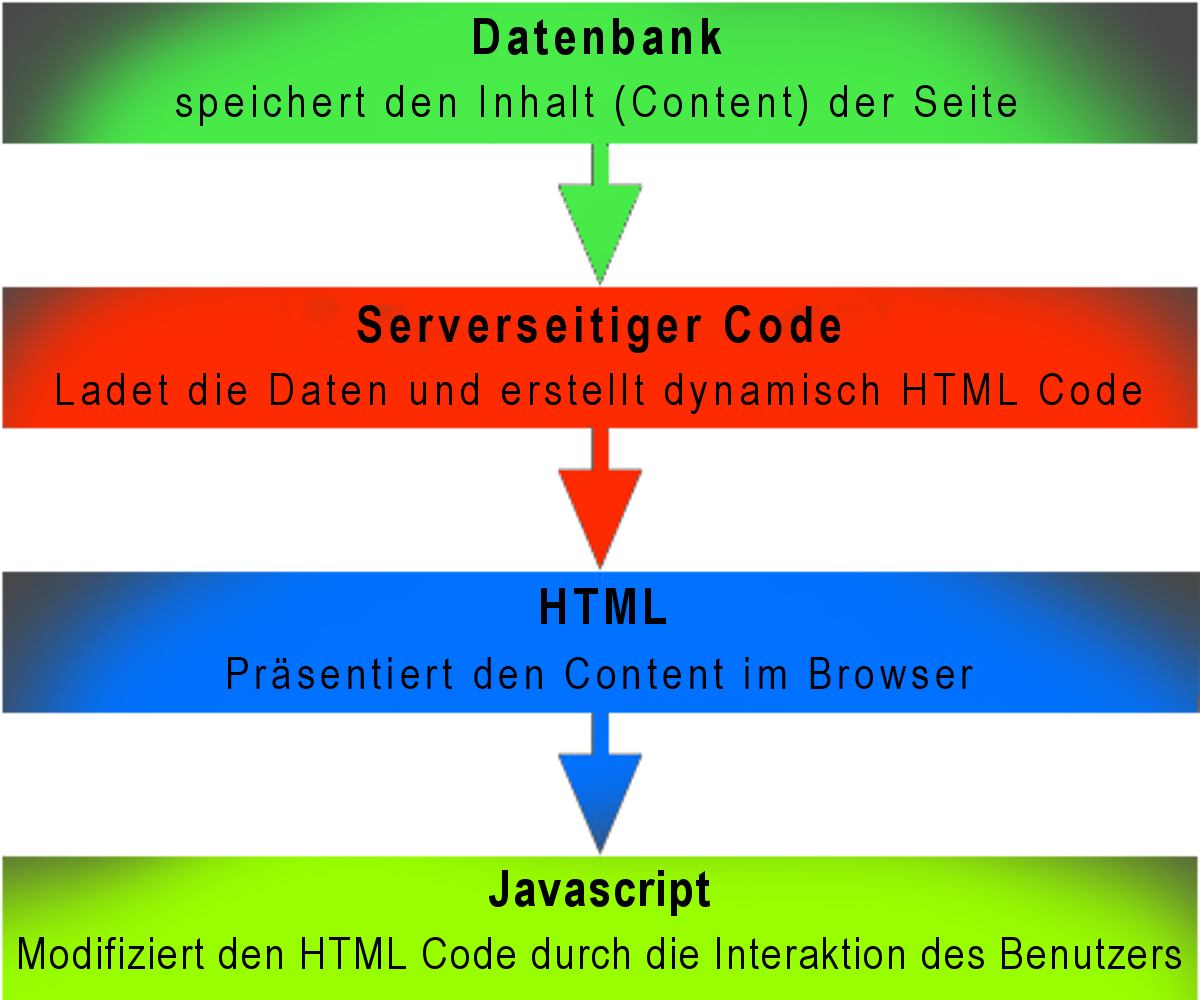
\includegraphics[width=300px]{Images/web-layers.png}
\caption{Aufbaukomponenten CMS}
\end{figure}
\newpage

\subsection{Webserver}

Um eine Webseite mit einer serverseitigen Sprache wie \acrshort{php} zu betreiben wird ein Webserver benötigt. Auf \gls{unix}-basierenden Servern ist dies meist Apache HTTP Server\footnote{http://httpd.apache.org (engl.)}. Auf Servern mit Windows Betriebssystemen ist dies im \acrshort{iis}-Packet\footnote{http://www.iis.net (engl.)} enthalten.

\begin{figure}[H]
	\centering
	\begin{subfigure}[b]{0.4\textwidth}
		
\includegraphics[width=\textwidth]{Images/iis.png}
		\caption{Internet Information Services}
	\end{subfigure}
	\begin{subfigure}[b]{0.4\textwidth}
		
\includegraphics[width=\textwidth]{Images/Apache_HTTP_Server.png}
		\caption{Apache HTTP Server}
	\end{subfigure}
    \caption{Webserver}
\end{figure}

\subsection{Script}

\begin{wrapfigure}{r}{110px}
\centering

\includegraphics[width=100px]{Images/php.png}
\caption{PHP}
\end{wrapfigure}

Für den Aufbau einer Website ist eine Vielzahl von Programmiersprachen zur Verfügung. Die am meisten verbreitete Sprache ist \acrshort{php}\footnote{http://www.php.net (engl.)}. \acrshort{php} ist ein System, das den Code serverseitig verarbeitet. Das bedeutet, dass der Quelltext nicht an den Webbrowser übermittelt wird, sondern an einen Interpreter auf dem Webserver. Erst die Ausgabe des \acrshort{php}-Interpreters wird an den Browser geschickt. In den meisten Fällen ist das ein \acrshort{html}-Dokument, wobei es mit \acrshort{php} aber auch möglich ist, andere Dateitypen, wie Bilder oder PDF-Dateien, zu generieren.

Mit dem Script wird das Grundgerüst für die Website erstellt. Das \acrshort{cms} steht als Grundgerüst als Download zur Verfügung.

\subsection{Datenbank}

Die Inhalte des \acrshort{cms} werden in kleinen Brocken in einer Datenbank gespeichert. Die meistverbreiteten Datenbanken sind MySQL\footnote{http://www.mysql.de} und PostgreSQL\footnote{http://www.postgresql.org (engl.)}. Auf den Windows Servern ist Microsoft SQL Server als Datenbank vorinstalliert. Zu beachten ist allerdings, dass die meisten \acrshort{cms} für eine spezifische Datenbankmanagementsoftware programmiert ist. Man kann sich daher nicht für eine beliebige Datenbank entscheiden, es sei denn das \acrshort{cms} unterstützt mehrere Datenbanken.

\begin{figure}[H]
	\centering
	\begin{subfigure}[b]{0.4\textwidth}
		
\includegraphics[width=100px]{Images/MySQL.png}
        \caption{MySQL}
	\end{subfigure}
	\begin{subfigure}[b]{0.4\textwidth}
		
\includegraphics[width=100px]{Images/postgresql.png}
    	\caption{PostgreSQL}
	\end{subfigure}
    
	\begin{subfigure}[b]{0.4\textwidth}
		
\includegraphics[width=100px]{Images/SQLite.png}
        \caption{SQLite}
	\end{subfigure}
	\begin{subfigure}[b]{0.4\textwidth}
		
\includegraphics[width=100px]{Images/mariadb.png}
    	\caption{MariaDB}
	\end{subfigure}
	\caption{gängige Datenbanksysteme}
\end{figure}

\subsection{Content Management System}

\subsubsection{WordPress}

\begin{wrapfigure}{r}{110px}
\centering

\includegraphics[width=100px]{Images/WordPress.png}
\caption{WordPress}
\end{wrapfigure}

WordPress ist eine freie Webanwendung zur Verwaltung der Inhalte einer Website (Texte und Bilder). Sie bietet sich besonders zum Aufbau und zur Pflege eines Weblogs (Blog) an, da sie jeden Beitrag einer oder mehreren frei erstellbaren Kategorien zuweisen kann und dazu automatisch die entsprechenden Navigationselemente erzeugt. Parallel kann WordPress auch hierarchische Seiten verwalten und gestattet den Einsatz als \gls{cms}.

Weiter bietet das System Leserkommentare mit der Möglichkeit, diese vor der Veröffentlichung erst zu prüfen, sowie eine zentrale Linkverwaltung, eine Verwaltung der Benutzerrollen und -rechte und die Möglichkeit externer Plugins, womit WordPress in Richtung eines vollwertigen CMS ausgebaut werden kann.

WordPress basiert auf der Programmiersprache \acrshort{php} und benötigt eine MySQL Datenbank um die Daten zu speichern. Laut Aussage der Entwickler legt das System besonderen Wert auf Webstandards, Eleganz, Benutzerfreundlichkeit und leichte Anpassbarkeit.

Vom Herunterladen des Pakets mit dem Quellcode bis zum fertigen Blog werden nach Entwicklerangaben weniger als fünf Minuten benötigt. Diese können sogar von Einsteigern häufig noch unterschritten werden.

WordPress unterstützt das Erstellen und Verwalten von Blog-Artikeln. Ausserdem ist standardmässig \acrshort{tinymce} als Texteditor aktiviert. Die Blog\textendash Beiträge werden neben der normalen Darstellung als Webseite den Lesern auch über Web\textendash Feeds z.B. \acrshort{rss} angeboten.

Mit Hilfe von \textbf{Plugins} kann WordPress um diverse Funktionen erweitert werden. Alle diese Erweiterungen lassen sich mittels des eingebauten Code-Editors bearbeiten.

Durch den Einsatz der \textbf{Themes}\textendash Technik werden Design und Programmkern von WordPress klar getrennt, was es leicht macht, individuelle Designs zu entwickeln, ohne mit der Programmierung der Software an sich vertraut zu sein. Allerdings ist es in WordPress auch möglich, diverse Funktionen direkt in ein Theme zu programmieren, wodurch diese Trennung teilweise wieder aufgehoben werden kann.

Ein normales WordPress\textendash Theme besteht aus einer Reihe von Bausteinen (PHP\textendash Funktionen) und \acrshort{html}\textendash Code. Jedes ''Theme'' folgt dabei einem grundlegend gleichen Aufbau. Daher gibt es von einigen Entwicklern spezielle Themes, die bereits alle grundlegenden Bausteine beinhalten und somit die Entwicklung eines eigenen ''Theme'' vereinfachen.
\newpage

\subsubsection{Typo3}

\begin{wrapfigure}{r}{110px}
\centering

\includegraphics[width=100px]{Images/Typo3.png}
\caption{Typo3}
\end{wrapfigure}

Als Datenbank kann MySQL oder MariaDB, aber auch PostgreSQL oder Oracle eingesetzt werden. Zahlreiche Funktionen von TYPO3 können mit Erweiterungen integriert werden, ohne dass ein eigener Programmcode geschrieben werden muss. Die derzeit über 5000 Erweiterungen stammen zum grössten Teil von Fremdanbietern und sind kostenlos verfügbar. Erhältlich sind unter anderem Erweiterungen für News, Shop\textendash Systeme oder Diskussionsforen.

TYPO3 \acrshort{cms} besteht, wie die meisten \acrshort{cms}, aus einem \gls{backend}, das der Pflege der Website dient, und einem \gls{frontend}, das die Website selbst darstellt.

Im \gls{backend} wird die Website verwaltet, konfiguriert, es werden Inhalte eingepflegt und bearbeitet. Ein \acrshort{wysiwyg}-Editor erlaubt es Anwendern ohne \acrshort{html}\textendash Kenntnisse, redaktionelle Tätigkeiten zu erledigen. Alternativ dazu kann die Bearbeitung von Inhalten auch direkt über das \gls{frontend} der Website vorgenommen werden. Diese Option bietet einen schnelleren Einstieg in das System.

\subsubsection{Joomla!}

\begin{wrapfigure}{r}{110px}
\centering

\includegraphics[width=100px]{Images/Joomla.png}
\caption{Joomla!}
\end{wrapfigure}
Joomla! ist in \acrshort{php} geschrieben und verwendet MySQL, MS SQL oder PostgreSQL als Datenbank.

Viele Anwender haben Erweiterungen für Joomla! erstellt, die sie der Nutzergemeinde meist kostenfrei zur Verfügung stellen \textemdash beispielsweise eine Online\textendash Shop\textendash Lösung. Auf diese Weise bietet Joomla! einen beachtlichen Funktionsumfang, der praktisch alle üblichen Anwendungen abdeckt. Neben den Vorteilen haben aber gerade diese Erweiterungen in der Vergangenheit immer wieder Sicherheitsprobleme hervorgerufen, so dass der Anwender eine gewisse Vorsicht walten lassen sollte. Zusätzlich zu den kostenfreien Erweiterungen gibt es auch einige kommerzielle Produkte für Joomla!, welche jedoch lizenzrechtlich umstritten sind.

Bei den Erweiterungen unterscheidet man Plugins, Komponenten, Module und Templates: Plugins verändern den Programmcode von Joomla!, Komponenten ergänzen zusätzliche Funktionalitäten, Module zeigen Daten aus dem Joomla!\textendash Kern oder anderen Erweiterungen an und die Templates bestimmen das Aussehen und die Seitenstruktur.

Aufgrund der Popularität und bekannter Sicherheitsprobleme werden Joomla!-Installationen immer wieder zur Zielscheibe von Angriffen, insbesondere in Form sogenannter \glspl{defacement}.

Im Entwicklerteam von Joomla! gibt es eine spezielle Abteilung, welche sich nur um das Auffinden von Fehlern (Bugs) kümmert und den Namen ''Bug Squad'' (Fehlerkommando) trägt. Vor allem die zahlreichen Drittkomponenten verursachen ein erhöhtes Sicherheitsrisiko, was von Hackern ausgenutzt wird. Viele \textemdash vor allem private \textemdash Benutzer vernachlässigen jedoch die Pflege einer Webseite und sind sich der resultierenden Probleme nicht bewusst.

\chapter{Aufbau des Systems}
\section{Installation Grundkomponenten}
Die zum Aufbau eines \acrshort{cms} benötigten Komponenten werden von der jeweiligen Website heruntergeladen und installiert. Alternativ können diese bei einem Windows Server auch im \gls{iis} mit den Webplatform\textendash Installer installiert werden.

\section{Konfiguration}
Die Konfiguration der Basiseinstellungen werden im \acrshort{iis} vorgenommen. Dazu wird eine neue Webseite erstellt und deren physikalischer Speicherort gewählt. Anschliessend wird eine \acrshort{ftp}\textendash Pubishing hinzugefügt, um später die Plugins der Website hinzufügen und aktualisieren zu können. Für das verwendete \acrlong{cms} werden neben dem System selber zusätzlich \acrshort{php} und MySQL benötigt.

\section{Installation CMS}

Aufgrund der Funktionalität, dem Umfang der Themes und Plugins sowie der Einfachheit des Programms. Ist die Wahl auf WordPress gefallen. Das Programm wird als \gls{zip}\textendash Datei von der Website geladen und entpackt. Die Dateien und Ordner werden in das zuvor definierte Verzeichnis verschoben.

Nach dem Verschieben kann der Installations\textendash Assistent gestartet werden, indem mit einem beliebigen Browser zu der Web\textendash Adresse navigiert wird. Dort wird nun die Verbindung zur MySQL\textendash Datenbank hergestellt und einige wenige Einstellungen für Wordpress vorgenommen.

Nachdem die Installation fertig ist, kann bereits mit dem Ausbau, dem Erstellen der Strukturen und Inhalten der Website begonnen werden.

\section{Menü\textendash Struktur}

Die Menü\textendash Struktur, der Aufbau des Menüs, ist hauptsächlich vom alten Intranet kopiert und beinhaltet alle wichtigen Punkte für die das informationelle Ziel eines Intranet.\\
\textendash Home\\
\textbar \textemdash Team\\
\textbar \textemdash \textemdash Organigramm\\
\textbar \textemdash Ressourcen\\
\textbar \textemdash \textemdash Trainingsvideos\\
\textbar \textemdash \textemdash Vorlagen\\
\textbar \textemdash \textemdash Protokolle\\
\textbar \textemdash \textemdash Kataloge\\
\textbar \textemdash \textemdash Bulletin\\
\textbar \textemdash ECDL\\
\textbar \textemdash Links\\

Einige der Menü\textendash Punkte enthalten Untermenüs um die verschiedenen Themen zu gruppieren. Auch werden einzelne Seiten in mehrere Unterseiten aufgeteilt.

Die Seite ''Home'' nutzt die Blog\textendash Funktion von Wordpress. Auf dieser Seite werden laufende Aktualitäten rund um den Betrieb und Themen wie Arbeitssuche, Gesundheit und Karriere publiziert.

\section{Meinungsumfrage}
Während rund 3 Wochen wurde bei der Geschäftsleitung und Mitarbeitern mit einer Umfrage nach der Meinung zum neuen Intranet gefragt.

Für die Stimmabgabe für Designs hatte jeder 2 Stimmen zur Verfügung und jeder konnte somit seine beiden Favoriten wählen. Wie in der nachstehenden Grafik festzustellen ist, sind die beiden Designs 1 und 5 die beiden Spitzenreiter. Das Design 1 mit dem Namen "Catch Responsive" wurde mit 24 Stimmen gewählt. Aufgrund von Inkompatibilität von grundlegenden Funktionen im Design 3 (Hemingway) wurde dieses vorzeitig aus dem Rennen genommen.

\begin{figure}[H]
\centering
\begin{tikzpicture}
\begin{axis}[xbar,
    y axis line style = { opacity = 0 },
    axis x line       = none,
    tickwidth         = 0pt,
    enlarge y limits  = 0.2,
    enlarge x limits  = 0.02,
    symbolic y coords = {Design 1, Design 2, Design 3, Design 4, Design 5},
    nodes near coords,
  ]
\addplot [draw=none, fill=orange!60] coordinates {

(20,Design 5)
(12,Design 4)
(0,Design 3)
(10,Design 2)
(24,Design 1)
};
\end{axis}
\end{tikzpicture}
\caption{Stimmenverteilung Themes}
\end{figure}

Während der Dauer der Umfrage wurden die vorgeschlagenen Designs rotierend aktiviert, damit jeder die Möglichkeit bekam diese auch Live ausprobiert werden konnten.
\newpage

Neben den Designs konnten die Mitarbeiter ihre Meinung auch zu den Inhalten des neuen Intranet angeben.


\begin{figure}[H]
\centering
\begin{tikzpicture}
\begin{axis}[
	xbar, axis on top,
    height=14cm, width=8cm,
    xmajorgrids, tick align=inside,
    major grid style={draw=black},
    y axis line style = { opacity = 0 },
    axis x line       = none,
    tickwidth         = 0pt,
    enlarge y limits  = 0.00,
    enlarge x limits  = 0.02,
    symbolic y coords = {Eintritt, Austritt, Abteilungen, Organigramm, Team, Vorlagen, Ein- und Austrittsdoku, Bulletins, Kataloge, Handbücher, Protokolle, ECDL, Links, Bewerbungstipps, Anderes},
    nodes near coords,
  ]
\addplot [draw=none, fill=orange!60] coordinates {
(4,Eintritt)
(5,Austritt)
(10,Abteilungen)
(6,Organigramm)
(14,Team)
(8,Vorlagen)
(4,Ein- und Austrittsdoku)
(8,Bulletins)
(10,Kataloge)
(6,Handbücher)
(4,Protokolle)
(6,ECDL)
(5,Links)
(12,Bewerbungstipps)
(2,Anderes)};
\end{axis}
\end{tikzpicture}
\caption{Stimmen pro Thema}
\end{figure}

\section{Themen der Inhalte}

Wie aus den Resultaten der Umfrage entnommen werden kann, wünschen sich viele Tipps zum Thema Bewerbung. Es existieren im Netz bereits sehr viele Blogs von Firmen, welche sich mit den Themen Bewerbung, Karriere und Gesundheit beschäftigen. Dies bietet die komfortable Möglichkeit, Beiträge aus diesen Blogs zu übernehmen. Als Quellenangabe werden diese durch einem Link am Ende des Beitrags zum Originalartikel verlinkt. Einige dieser Blogs sind in englischer Sprache verfasst. Die Beiträge dieser Blogs werden für die Verwendung im Intranet ins Deutsche übersetzt.

Nachstehend ist eine Auswahl der Blogs, von welchen die Beiträge übernommen werden.

\begin{table}[H]
\centering
\begin{tabular}{ l l l }
JobScout24    	& http://jobscout24.ch/de/jobratgeber	&\\
Beobachter		& http://beobachter.ch/arbeit-bildung	&\\
Karriere        & http://karriere.ch					&\\
Monster         & http://karriere-journal.monster.ch	&\\
Karrieretipps   & http://karrieretipps.de				&\\
Jobs.ch         & http://jobs.ch/de/tipps				&\\
Kununu          & http://news.kununu.com				&\\
Edition F		& http://editionf.com					&\\
Careerbuilder   & http://advice.careerbuilder.com		& 
\includegraphics[width=22px]{Images/en_GB.png}\\
jobspotting		& http://jobspotting.com				& 
\includegraphics[width=22px]{Images/en_GB.png}\\
Lifehack		& http://lifehack.org					& 
\includegraphics[width=22px]{Images/en_GB.png} 
\end{tabular}
\caption{Links zu Blogs}
\end{table}



\chapter{Themes}
\section{Auswahl des Themes}
Für das Intranet wurden 5 verschiedene Designs zur Auswahl ausgesucht. Diese waren sowohl im Aussehen als auch in deren Funktionalität sehr unterschiedlich. Während den ersten Tests mit den verschieden Designs wurde allerdings klar das das Design 3 (Hemingway) mit einem Teil der bereits programmierten Inhalte nicht kompatibel war. Die Vorlage wurde noch während der Umfrage ersatzlos aus den Vorschlägen gestrichen.

Sowohl auf der Website von WordPress als auch bei anderen Anbietern sind total ungefähr 10'000 verschiedene Themes verfügbar. Diese können mit geringstem Aufwand installiert und aktiviert werden. Sehr viele davon sind optisch wie auch funktionell auf nöchstem Niveau und sind auf für die Darstellung auf verschiedenen Geräten (Computer, Tablett, Smartphone) ausgerichtet. Diese reaktive Anpassung an die verschiedenen Bildschirmgrössen wird "\gls{rwd}" genannt.
\newpage

\section{Funktionen}

Die verschiedenen Designs kommen mit verschiedenen zum Teil gemeinsamen, zum Teil aber auch einzigartigen Features und Funktionen. Nachstehend eine Auswahl der Funktionen der 5 gewählten Designs:

\begin{itemize}
\item Promotion-überschrift (Catch Responsive)
\item Slider (Catch Responsive, Grow, Spacious)
\item Vorgestellter Inhalt (Catch Responsive, Grow)
\item Suche ein- oder ausblenden
\item Kopfbild festlegen
\item Statisches Hintergrundbild
\item Festsetzen von Akzentfarben
\end{itemize}

\section{Theme-Vorschläge}

\begin{figure}[H]
\centering
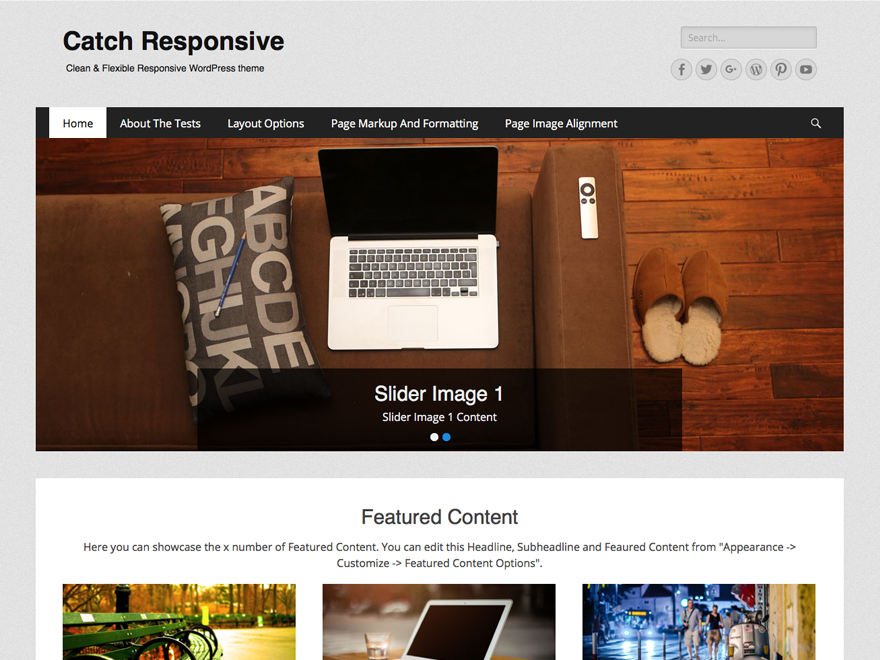
\includegraphics[width=300px]{Images/Design_1.png}
\caption{Design 1 - Catch Responsive}
\end{figure}
\begin{figure}[H]
\centering
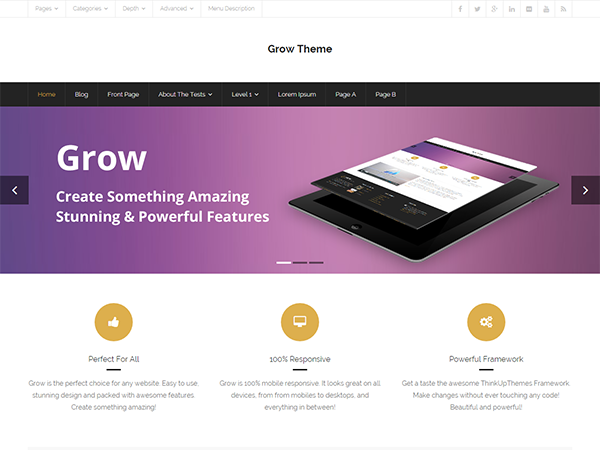
\includegraphics[width=300px]{Images/Design_2.png}
\caption{Design 2 - Grow}
\end{figure}
\begin{figure}[H]
\centering
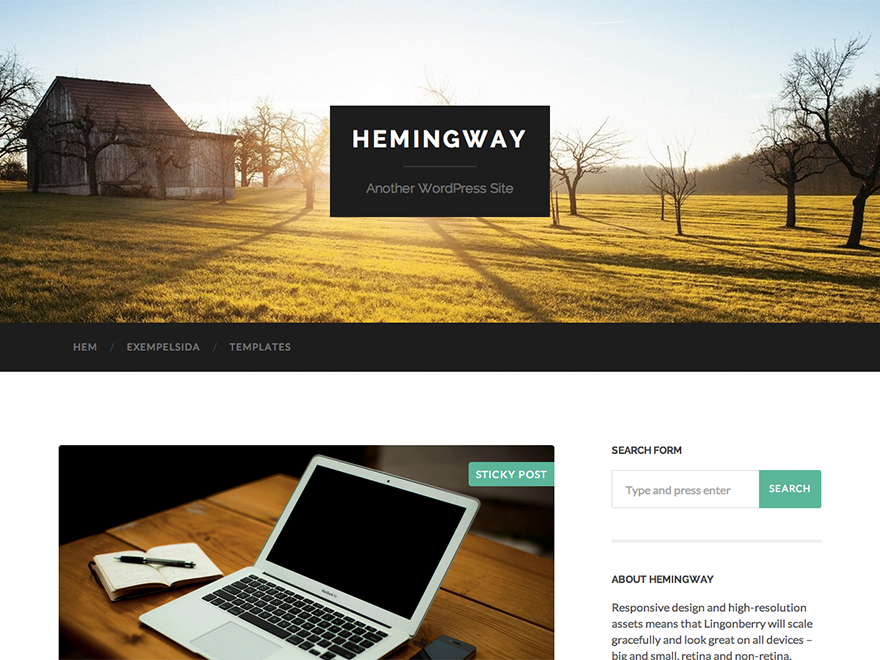
\includegraphics[width=300px]{Images/Design_3.png}
\caption{Design 3 - Hemingway}
\end{figure}
\begin{figure}[H]
\centering
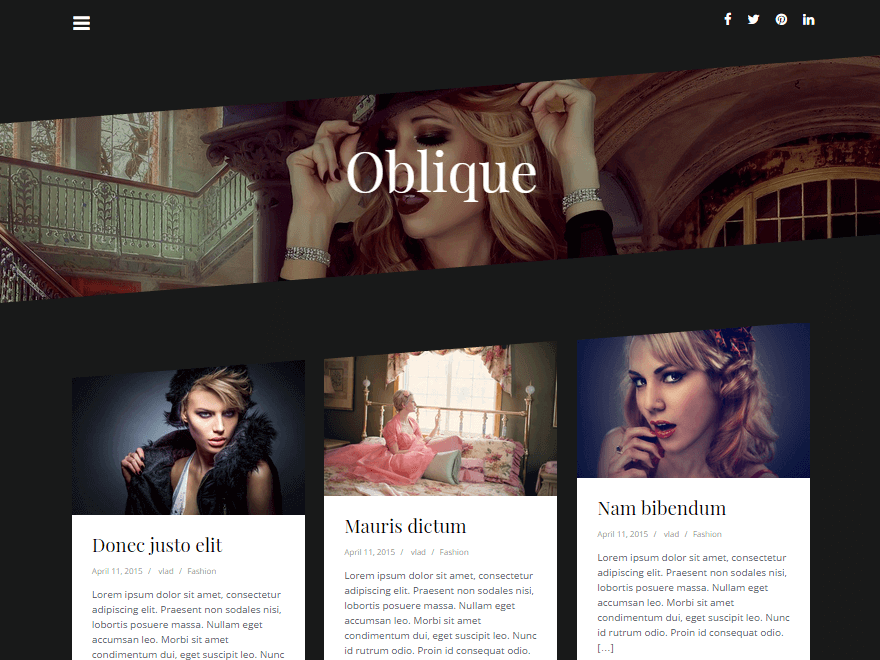
\includegraphics[width=300px]{Images/Design_4.png}
\caption{Design 4 - Oblique}
\end{figure}
\begin{figure}[H]
\centering
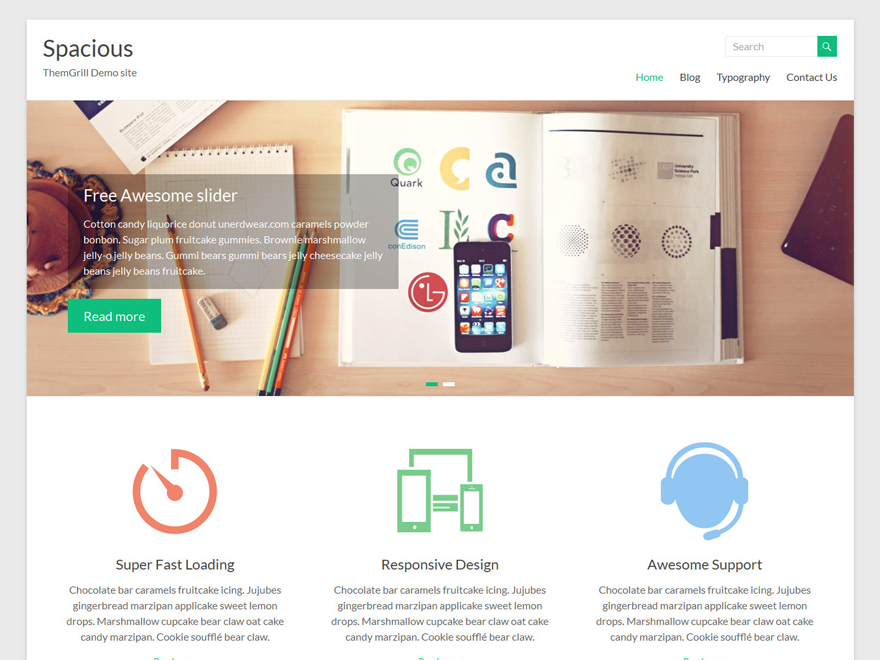
\includegraphics[width=300px]{Images/Design_5.png}
\caption{Design 5 - Spacious}
\end{figure}


\chapter{Plugins}

WordPress bietet über 40'000 Plugins um eine Website um jede beliebige Funktion zu erweitern. Die Vielfalt kommt auch dem Intranet zugute. So wurden einige dieser Plugins integriert um eine möglichst einfache Bedienung zu garantieren oder um zusätzlichen Nutzen für die Mitarbeiter zu generieren.

\section{Shortcode}

Ein Shortcode ist ein WordPress-spezifischer Code, mit dem man raffinierte Dinge mit sehr wenig Aufwand machen kann. Shortcodes können Dateien einbetten oder mit nur einer Zeile Objekte erstellen, die normalerweise viel komplizierten, hässlichen Code erfordern würden. Ein Shortcode kann etwas wie ein Shortcut (engl. für Abkürzung) angesehen werden.

\section{Active Directory/LDAP Login for Intranet sites}

\begin{wrapfigure}{R}{120px}
\vspace{-20px}
\centering

\includegraphics[width=100px]{Images/ldap.png}
\caption{miniOrange}
\end{wrapfigure}

Das Plugin bietet Login zu WordPress durch Anmeldeinformationen, welche in einem \acrshort{ldap}-Server (wie Microsoft Active Directory oder Open\acrshort{ldap}) gespeichert sind. So ist es möglich sich mit dem eigenen Vor- und Nachnamen und dem Windows-Passwort anzumelden, ohne ein zusätzliches Passwort zu merken zu müssen.\par
\newpage
Die Konfiguration des Plugins erfolgt über den Reiter \acrshort{ldap} Configuration. Format der Server-Adresse: ldap://192.168.1.1:389\\
Anschliessend wird die \acrshort{ldap} User Mapping Configuration durchgeführt. Dies definiert in welchem Teil des Directory die User gesucht werden:\\ ou=department,dc=company,dc=local\\
Nun kann die Verbindung mit Benutzername und Kennwort hergestellt werden.

\section{Artikel duplizieren}

\begin{wrapfigure}{r}{120px}
\vspace{-20px}
\centering

\includegraphics[width=100px]{Images/duplicate.png}
\caption{Duplicate}
\end{wrapfigure}

Für die Benachrichtigung über Neueintritte und Abteilungswechsel wird immer wieder die gleiche Beitragsstruktur verwendet. Um diese Duplikate einfacher zu erstellen und zu verwalten, wurde dieses Plugin installiert. Es erlaubt mit einem einzelnen Klick, einen beliebigen Post zu duplizieren, welcher anschliessend nur noch inhaltlich angepasst werden muss.


\section{Media Library Plus}

\begin{wrapfigure}{r}{120px}
\vspace{-20px}
\centering

\includegraphics[width=100px]{Images/Media_Library_Plus.jpg}
\caption{Media Library Plus}
\vspace{-10px}
\end{wrapfigure}

WordPress speichert Medien, welche auf die Seite geladen werden in der Ordnerstrucktur wp-content/ uploads/JAHR/MONAT wobei die Dateien in der Mediathek unsortiert dargestellt werden.

Das Plugin ermöglicht es die Medien in spezifische Ordner zu speichern und zu sortieren. So können alle PDF-Dokumente gemeinsam in einen Ordner gespeichert werden.

Weiter bietet das Plugin auch die Möglichkeit Bilder und Dokumente umzubenennen und in andere Ordner zu verschieben. Die ''normale'' Media Library wird durch dieses Plugin nicht ersetzt sondern ergänzt.
\newpage

\section{Quiz And Survey Master}

\begin{wrapfigure}{r}{120px}
\vspace{-20px}
\centering

\includegraphics[width=100px]{Images/Quiz_Survey_Master.png}
\caption{Media Library Plus}
\vspace{-10px}
\end{wrapfigure}

Mit dem Quiz und Survey Master können Umfragen und Quiz erstellt werden. Es ist möglich, anhand der erreichten Punkte unterschiedliche End-Seiten zu erstellen. Damit lässt sich so zum Beispiel eine Erklärung zu dem Resultat für eine Typenauswertung einbauen.

Weiter hat mann die Möglichkeit, mittels eMail-Benachrichtigung über neue Daten informiert zu werden. Mit den kostenpflichtigen Premium Addon kann dieses Plugin noch erweitert werden.

Dieses Plugin hat bisher noch keine Anwendung erhalten und ist daher noch inaktiv. Es kann jedoch jederzeit aktiviert und direkt eingesetzt werden.

\section{TinyMCE Advanced}

\begin{wrapfigure}{r}{120px}
\vspace{-20px}
\centering

\includegraphics[width=100px]{Images/TinyMCE.png}
\caption{TinyMCE Advanced}
\vspace{-10px}
\end{wrapfigure}

\acrshort{tinymce} ist ein \acrshort{wysiwyg}-Editor welcher es möglich ist, ohne \acrshort{html}-Kenntnisse Seiten und Beiträge zu verfassen. Die Standard-Version ist bereits im WordPress installiert. Dieses Plugin erweitert diesen Editor mit weiteren Funktionen:

\begin{itemize}
\item Erstellen von Tabellen
\item Mehr Optionen zum erstellen von Listen
\item Suchen und Ersetzen
\item Möglichkeit die Schriftart und Schriftgrösse zu definieren
\item und einiges Mehr
\end{itemize}


\section{Quote Master}

Diesem Plugin liegt eine Liste von Zitaten (Quotes) zugrunde. Diese Zitate können beliebig erfasst und ergänzt werden. Das Plugin wird als \gls{widget}, beispielsweise in der Seitenleiste der Website eingebaut. Die Quotes werden nach dem Zufallsprinzip in einer Box publiziert.

\begin{figure}[H]
\centering
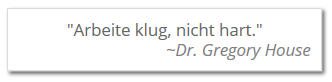
\includegraphics[width=250px]{Images/quote.png}
\caption{Quote}
\end{figure}

\section{Slideshow}

\begin{wrapfigure}{r}{120px}
\vspace{-20pt}
\centering

\includegraphics[width=100px]{Images/slideshow.png}
\caption{Slideshow}
\vspace{-20pt}
\end{wrapfigure}

Mit einer Slideshow können Bilder als rotierende Galerie auf einer beliebigen Seite eingebunden werden. Dies ist vor allem für Events gedacht zu welchem mehrere Bilder in einem Blogbeitrag oder einer Seite publiziert werden möchten. Der Shortcode für das Einbinden wird vom Plugin erstellt:

\lstset{language=html}
\begin{lstlisting}[frame=single]
Shortcode = [slideshow_deploy id='123']
\end{lstlisting}

\section{SOUP - Show Off Upcoming Posts}

\begin{wrapfigure}{r}{120px}
\vspace{-20pt}
\centering
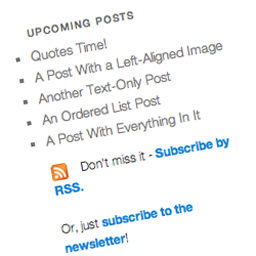
\includegraphics[width=100px]{Images/soup.png}
\caption{SOUP}
\vspace{-10pt}
\end{wrapfigure}

SOUP ist ein kleines Plugin, welches zukünftige, geplante Beiträge als Liste von 3 bis 5 Elementen als \gls{widget} in die Website einbindet. Die Liste kann mit einigen Einstellungen bearbeitet werden. So kann entschieden werden wie viele Beiträge angezeigt werden, ob das Veröffentlichungsdatum angezeigt wird und ob die Elemente in chronologischer oder zufälliger Reihenfolge dargestellt werden.

\section{Team Members}
\begin{wrapfigure}{r}{120px}
\vspace{-20pt}
\centering

\includegraphics[width=100px]{Images/Team_Members.png}
\caption{Team Members}
\end{wrapfigure}
Das Plugin Team Members zeigt eine Auflistung der Mitarbeiter an. Auf diese Weise können Personen mit Foto, eMail und anderen Infos auf einer Seite abgebildet werden.

Eingebaut werden die verscheidenen Mitarbeiterlisten über den Shortcode, welchen das Plugin zur jeweiligen Liste generiert:

\lstset{language=html}
\begin{lstlisting}[frame=single]
Shortcode = [tmm name="abc123"]
\end{lstlisting}

Durch Verwendung von \acrshort{html}-Code ist es möglich Bilder, z.B. Flaggen in die Profile einzubinden oder den Text zu formatieren.:

\lstset{language=html}
\begin{lstlisting}[frame=single]
<img src="wp-content/Uploads/Flags/de_CH.gif" alt="de_CH"
title="Schweizerdeutsch" height="36" width="22">
\end{lstlisting}

\begin{wrapfigure}{r}{120px}
%\vspace{-20pt}
\centering
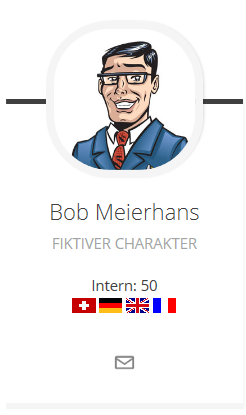
\includegraphics[width=100px]{Images/Teammember.png}
\caption{Ansicht Team Member}
%\vspace{-10pt}
\end{wrapfigure}

Dieser Code resultier in einer kleinen Schweizer Flagge mit einer Höhe (\textbf{height}) von 22 \gls{pixel} und einer Breite (\textbf{width}) von 36 \gls{pixel}. \textbf{src} (engl. source / Quelle) bezieht sich auf den Speicherort der Grafik. \textbf{alt} (engl. alternative) gibt den Alternativtext an, der angezeigt wird, wenn das Bild nicht geladen werden kann. \textbf{title} beschreibt ein Element. Browser blenden diesen Text ein, wenn der Anwender das Element hovert (mit der Maus draufzeigt).

Um die Flagge anderer Sprachen einzufügen müssen die beiden Werte ''de\_CH'' in den entsprechenden Sprachencode sowie ''Schweizerdeutsch'' in der Name der Sprache geändert werden. Wenn neue Sprachen hinzukommen, wird die Flagge mit Ausmassen 630 x 420 \gls{pixel} im Format \acrshort{gif} erstellt und mit dem Media Library Plus im Ordner ''Flags'' gespeichert.
\newpage

Die Flaggen folgender Länder resp. Sprachen sind programmiert:

\begin{table}[H]
\centering
\begin{tabular}{ l p{2.5cm} c }
Sprache 			& Sprachcode \& Filename	& Flagge\\
Schweizerdeutsch	& de\_CH		& 
\includegraphics[width=22px]{Images/de_CH.png}\\
Deutsch				& de\_DE		& 
\includegraphics[width=22px]{Images/de_DE.png}\\
Englisch			& en\_GB		& 
\includegraphics[width=22px]{Images/en_GB.png}\\
Französisch			& fr\_FR		& 
\includegraphics[width=22px]{Images/fr_FR.png}\\
Italienisch			& it\_IT		& 
\includegraphics[width=22px]{Images/it_IT.png}\\
Albanisch			& sq\_AL		& 
\includegraphics[width=22px]{Images/sq_AL.png}\\
Spanisch         	& es\_ES		& 
\includegraphics[width=22px]{Images/es_ES.png}\\
Türkisch			& tr\_TR		& 
\includegraphics[width=22px]{Images/tr_TR.png}\\
Kurdisch			& ku\_IQ		& 
\includegraphics[width=22px]{Images/ku_IQ.png}\\
\end{tabular}
\caption{Ländercodes}
\end{table}

\section{Editorial Calendar}

Um die Beiträge übersichtlich darzustellen und deren Veröffentlichung einfach zu koordinieren, wurde der Editorial Kalender installiert. Auf einem Monatskalender werden die zukünftig geplanten Beiträge angezeigt. Zusätzlich sind in einer Liste jene Beiträge ersichtlich, welche noch nicht terminiert wurden.

\begin{figure}[H]
\centering
\vspace{+20px}
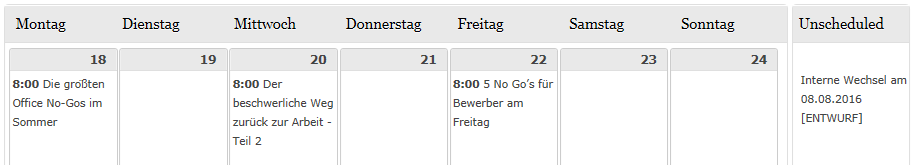
\includegraphics[width=\textwidth]{Images/Calendar.png}
\caption{Editorial Kalender}
\end{figure}
\newpage

\section{Football Pool}

\begin{wrapfigure}{r}{120px}
\vspace{-20px}
\centering

\includegraphics[width=100px]{Images/Football_Pool.png}
\caption{Football Pool}
\vspace{-10px}
\end{wrapfigure}


Für die Euro 2016 wurde ein Tipp-Spiel auf dem Intranet eingebaut. Vor jedem Match konnten die Teilnehmenden ihre Prognose eintragen und erhielten anschliessend anhand des Endresultats Punkte gutgeschrieben.

Hat ein Spieler für das Spiel Deutschland vs. Frankreich einen Tipp 2:0 abgegeben und das Spiel endete mit 2:1 erhielt man anhand der nachstehenden Tabelle 2 Punkte für den richtigen Sieger und 3 Punkte für das vorhersagen der Tore auf einer Spielseite (in diesem Beispiel die 2 Tore von Deutschland).

\begin{table}[H]
\centering
\begin{itemize}
\item 5 Pkt - Richtiges Endergebnis
\item 2 Pkt - Richtiges Sieger
\item 3 Pkt - Torbonus
\item 2 Pkt - Richtige Tordifferenz
\item 3x - Joker Multiplikator 
\end{itemize}
\caption{Punkteverteilung}
\end{table}

Dieses Plugin gilt als ein Beispiel, wie man das Intranet auch in Zufunft dynamisch an bestimmte Events von allgemeinem Interesse verändern kann und eine Möglichkeit, wie Mitarbeiter gerne zur Arbeit kommen\footnote{https://www.entrepreneur.com/article/246981}.

\chapter{Content Management}
\section{Benutzerrollen}

WordPress kennt 5 verschiedene Benutzerrollen. Jede hat unterschiedliche Fähigkeiten und Befugnisse, angefangen beim Leser mit keinerlei Rechten bis zum Administrator mit allen Rechten.

\begin{table}[H]
\centering
\begin{itemize}
\item \textbf{Administrator}\\ hat Zugang zu allen Funktionen der Seite
\item \textbf{Redaktor} (Editor)\\ kann Posts publizieren und verwalten, inklusive Posts von anderen
\item \textbf{Autor} (Author)\\ kann eigene Posts publizieren und verwalten, nicht aber jene von anderen Verfassern
\item \textbf{Mitarbeiter} (Contributor)\\ kann eigene Posts schreiben und verwalten, nicht aber publizieren
\item \textbf{Leser} (Subscriber)\\ kann nur lesen und das eigene Profil verwalten
\end{itemize}

\caption{Benutzerrollen und deren Rechte}
\end{table}

Um die Sicherheit und Integrität des Systems, Vorlagen und der Konfiguration zu gewährleisten ist es wichtig, dass so weit wie möglich der Zugang zu den empfindlichen Einstellungen eingeschränkt bleibt. Aber es ist auch erforderlich, dass die verschiedenen Abteilungen einen, wenn auch limitierten, Zugang zum \gls{backend} erhalten. Dies vor allem um die anfallenden Arbeiten zur Pflege des Intranets aufzuteilen.

\begin{figure}[H]
\centering
\vspace{+20px}
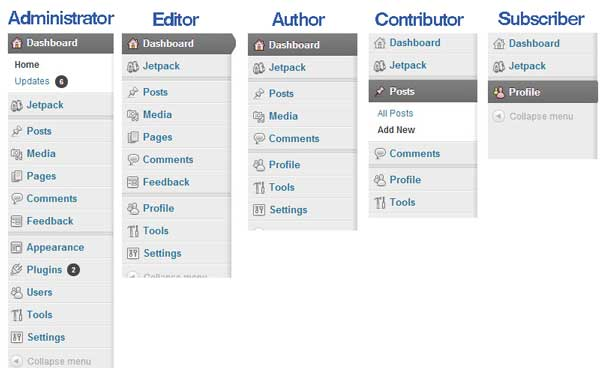
\includegraphics[width=\textwidth]{Images/userroles.jpg}
\caption{WordPress Ansicht der Benutzerrechte}
\end{figure}

Die Zugänge mit Administrator- und Redaktor-Rechten bleiben dafür bei der Abteilung Informatik, der Geschäftsleitung und gegebenenfalls einzelne Abteilungsleiter. Zugänge auf den Stufen Autor und  Mitarbeiter können in den Abteilungen Marketing (zum Promoten der Flyer, Bulletins etc.) und Personal (Eintrittsmeldungen) vergeben werden. Es ist dabei immer abzuwägen wie viele Rechte diese Zugänge bekommen sollen. Eine genaue Übersicht, welche Rechte die verschiedenen Benutzerrollen haben ist auf wordpress.org\footnote{http://codex.wordpress.org/roles\_and\_capabilities (engl.)} aufgelistet. Dort ist zu beachten, dass in der installierten Version die Rolle ''Super Admin'' nicht gibt und dessen Rechte der Rolle ''Administrator'' zugeteilt sind.

\section{Schulung}

\begin{wrapfigure}{r}{120px}
\centering

\includegraphics[width=100px]{Images/vimeo.png}
\caption{Vimeo}
\end{wrapfigure}
Um eine anhaltende Sicherstellung der Pflege des Intranets sicherzustellen, sind zweierlei Arten von Schulungskonzepten vorgesehen.

Zum einen werden für die verschiedenen Aufgaben jeweils Schritt-für-Schritt Anleitungen erstellt. Diese Dokumente beinhalten zum Beispiel die genauen Grössen und Dateiformate für die zu verwendenden Bilder oder die Art und Weise wie ein \acrshort{pdf} Katalog, Flyer oder Bulletin erstellt werden soll, um ein gleichbleibend hochstehendes Qualitätsniveau zu halten.

Zum andern werden für diese Abläufe als Video dokumentiert und über die Videoplattform Vimeo\footnote{http://www.vimeo.com} in der Rubrik Ressourcen \ding{213} Trainingsvideos im Intranet eingebunden. Die Dokumentation dieser Abläufe mittels Videos bietet den Vorteil, dass Kleinigkeiten, welche in den schriftlichen Anleitungen nicht beachtet wurden, sichtbar bleiben, so dass die Vorgänge leicht verständlich sind.

Für Allpower besteht ein Vimeo-Account\footnote{http://www.vimeo.com/allpower}, wo die Videos gespeichert werden. Über diese \acrshort{url} können die Videos auch von Zuhause aus betrachtet werden. Aus diesem Grund ist speziell darauf zu achten, dass persönliche Daten von Mitarbeitern oder sensible geschäftliche Daten nicht in diesen Videos erscheinen, respektive diese zensiert werden.

\setglossarystyle{altlist}
\printglossaries
\cleardoublepage
\pagestyle{empty}
\vspace*{\fill}
\begin{center}
Copyright \copyright \ 2016 Christian Seiler \\
Alle Rechte vorbehalten.\\
\LaTeX
\end{center}
%%% End document
\end{document}